\documentclass[UTF8]{ctexart}
\usepackage{graphicx}
\usepackage{amsmath}

\title{\heiti 变分原理及有限元大作业}
\author{SX1501021 仓宇}
\date{\today}

\bibliographystyle{plain}

\begin{document}
\maketitle

\clearpage

\tableofcontents

\clearpage

\section{问题描述}
求解如图所示的平面钢架的节点位移和内力,各杆材料和几何尺寸均相同。$E=2\times10^7N/cm^2$,$l=100cm$,$A=10cm^2$,$Iz=25cm^4$,$P=10000N$。
\begin{center}
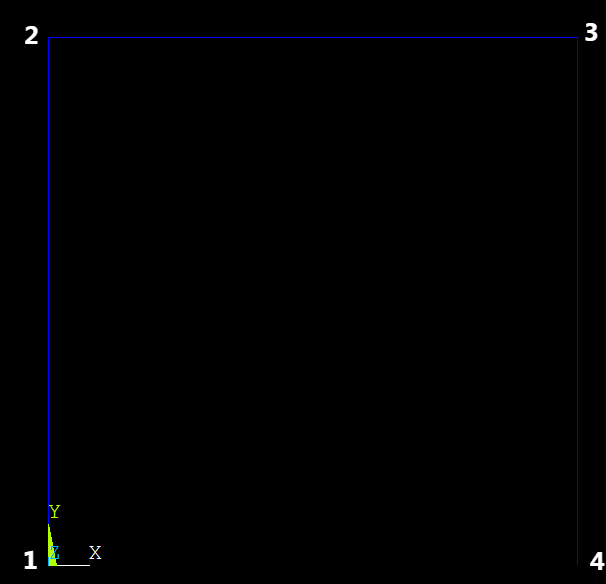
\includegraphics[width=8cm]{ScreenClip-1.png}
\end{center}

\section{计算局部刚度矩阵}
节点位移包括节点沿X、Y方向的位移和绕Z轴的转角,采用2节点的插值方式。局部刚度矩阵如下:
\[ \overline{K^e}= \begin{pmatrix}
	\frac{EA}{l} & 0 & 0 & \frac{-EA}{l} & 0 & 0 \\
    	0 & \frac{12EIz}{l^3} & \frac{6Iz}{l^2} & 0 & \frac{-12EIz}{l^3} & \frac{6EIz}{l^2} \\
    	0 & \frac{6EIz}{l^2} & \frac{4EIz}{l} & 0 & \frac{-6EIz}{l^2} & \frac{2EIz}{l} \\
    	\frac{-EA}{l} & 0 & 0 & \frac{EA}{l} & 0 & 0\\
    	0 & \frac{-12EIz}{l^3} & \frac{-6EIz}{l^2} & 0 & \frac{12EIz}{l^3} & \frac{-6EIz}{l^2} \\
    	0 & \frac{6EIz}{l^2} & \frac{2EIz}{l} & 0 & \frac{-6EIz}{l^2} & \frac{4EIz}{l}
\end{pmatrix} \]

将各个参数代入,计算结果如下:

\[ \overline{K^1}=\overline{K^2}=\overline{K^3}= \begin{pmatrix}
2000000 &	0 &	0 &	-2000000 &	0 &	0 \\
0 &	6000 &	300000 &	0 &	-6000 &	300000 \\
0 &	300000 &	20000000 &	0 &	-300000 &	10000000 \\
-2000000 &	0 &	0 &	2000000 &	0 &	0 \\
0 &	-6000 &	-300000 &	0 &	6000 &	-300000 \\
0 &	300000 &	10000000 &	0 &	-300000 &	20000000 \\
\end{pmatrix} \]

\section{计算全局刚度矩阵}

首先确定全局坐标系在各个局部坐标系下的方向余弦系数,得到的变换矩阵如下:

\[ \lambda^1= \begin{pmatrix}
0 &	1 &	0 &	0 &	0 &	0 \\
-1 &	0 &	0 &	0 &	0 &	0 \\
0 &	0 &	1 &	0 &	0 &	0 \\
0 &	0 &	0 &	0 &	1 &	0 \\
0 &	0 &	0 &	-1 &	0 &	0 \\
0 &	0 &	0 &	0 &	0 &	1 
\end{pmatrix} \]

\bigskip

\[ \lambda^2= \begin{pmatrix}
1 &	0 &	0 &	0 &	0 &	0 \\
0 &	1 &	0 &	0 &	0 &	0 \\
0 &	0 &	1 &	0 &	0 &	0 \\
0 &	0 &	0 &	1 &	0 &	0 \\
0 &	0 &	0 &	0 &	1 &	0 \\
0 &	0 &	0 &	0 &	0 &	1 
\end{pmatrix} \]

\bigskip

\[ \lambda^3= \begin{pmatrix}
0 &	-1 &	0 &	0 &	0 &	0 \\
1 &	0 &	0 &	0 &	0 &	0 \\
0 &	0 &	1 &	0 &	0 &	0 \\
0 &	0 &	0 &	0 &	-1 &	0 \\
0 &	0 &	0 &	1 &	0 &	0 \\
0 &	0 &	0 &	0 &	0 &	1 
\end{pmatrix} \]

根据局部刚度矩阵与全局刚度矩阵之间的转换公式$K^e=\lambda^T \times \overline{K^e} \times \lambda$,得到各个单元在全局坐标系下的刚度矩阵为如下:

\[ K^1= \begin{pmatrix}
        6000 &           0 &     -300000  &      -6000    &        0   &   -300000 \\
           0 &     2000000     &       0   &         0   &  -2000000    &        0 \\
     -300000  &          0    & 20000000  &     300000 &          0  &   10000000 \\
       -6000  &          0     &  300000     &    6000  &          0    &   300000 \\
           0  &   -2000000    &        0    &        0    &  2000000  &          0 \\
     -300000     &       0   &  10000000      & 300000     &       0 &    20000000

\end{pmatrix} \]

\bigskip

\[ K^2= \begin{pmatrix}
     2000000    &        0  &          0 &    -2000000  &          0   &         0 \\
           0    &     6000  &     300000  &          0   &     -6000   &    300000 \\
           0    &   300000  &   20000000  &          0  &    -300000 &    10000000 \\
    -2000000     &       0   &         0   &   2000000   &         0  &          0 \\
           0     &   -6000   &   -300000   &         0  &       6000  &    -300000 \\
           0   &    300000   &  10000000   &         0  &    -300000  &   20000000

\end{pmatrix} \]

\bigskip

\[ K^3= \begin{pmatrix}
        6000   &         0     &  300000  &      -6000  &          0 &      300000 \\
           0    &  2000000   &         0  &          0  &   -2000000 &           0 \\
      300000    &        0  &   20000000  &    -300000  &          0 &    10000000 \\
       -6000   &         0    &  -300000  &       6000  &          0 &     -300000 \\
           0  &   -2000000  &          0   &         0 &     2000000 &           0 \\
      300000    &        0  &   10000000   &   -300000  &          0 &    20000000

\end{pmatrix} \]

\section{组集结构刚度矩阵}

由于本例结构较为简单,将各个单元的全局刚度矩阵按照对应的节点外载荷组集起来时只需要沿对角线放置上去即可,结构刚度矩阵K初始全设为0,
将单元1的刚度矩阵加在从(1,1)到(6,6)的对角方阵上,单元2的刚度矩阵加在从(4,4)到(9,9)的对角方阵上,单元3的刚度矩阵放在从(7,7)到(12,12)的对角方阵上。
最终得到的结果如下所示:

\[ K= \begin{pmatrix}
\begin{smallmatrix}
6000 & 0 & -300000 & -6000 & 0 & -300000 & 0 & 0 & 0 & 0 & 0 & 0 \\
0 & 2000000 & 0 & 0 & -2000000 & 0 & 0 & 0 & 0 & 0 & 0 & 0 \\
-300000 & 0 & 20000000 & 300000 & 0 & 10000000 & 0 & 0 & 0 & 0 & 0 & 0 \\
-6000 0 & 300000 & 2006000 & 0 & 300000 & -2000000 & 0 & 0 & 0 & 0 & 0 \\
0 & -2000000 & 0 & 0 & 2006000 & 300000 & 0 & -6000 & 300000 & 0 & 0 & 0 \\
-300000 & 0 & 10000000 & 300000 & 300000 & 40000000 & 0 & -300000 & 10000000 & 0 & 0 & 0 \\
0 & 0 & 0 & -2000000 & 0 & 0 & 2006000 & 0 & 300000 & -6000 0 & 300000 \\
0 & 0 & 0 & 0 & -6000 &-300000 & 0 & 2006000 & -300000 & 0 & -2000000 & 0 \\
0 & 0 & 0 & 0 & 300000 & 10000000 & 300000 & -300000 & 40000000 & -300000 & 0 & 10000000 \\
0 & 0 & 0 & 0 & 0 & 0 & -6000 & 0 &-300000 &6000 & 0 &-300000 \\
0 & 0 & 0 & 0 & 0 & 0 & 0 & -2000000 & 0 & 0 & 2000000 & 0 \\
0 & 0 & 0 & 0 & 0 & 0 & 300000 & 0 & 10000000 & -300000 & 0 & 20000000
\end{smallmatrix}
\end{pmatrix} \]

\section{求解节点位移与应力}

求得上述结构刚度矩阵后就可以代入已有载荷算出在节点2和节点3出的位移了,继而可算出在节点1和节点4处的约束反力。

\smallskip

 最终得到的位移和如下:
\begin{center}
$u_2=1.19356041537694$ \\
$v_2=0.00214102198115903$ \\
$\varphi_2=-0.00719205100884593$ \\
$u_3=1.19106228897174$ \\
$v_3=-0.00214102198115903$ \\
$\varphi_3=-0.00716706974479397$
\end{center}

\smallskip

最终得到的约束反力如下:
\begin{center}
$F_1x=-5003.74718960785$ \\
$F_1y=-4282.04396231806$ \\
$M_1=286147.614524622$ \\
$F_2x=-4996.25281039226$ \\
$F_2y=4282.04396231806$ \\
$M_2=285647.989243583$
\end{center}

通过Ansys验算得到的钢架位移结果如下所示:
\begin{center}
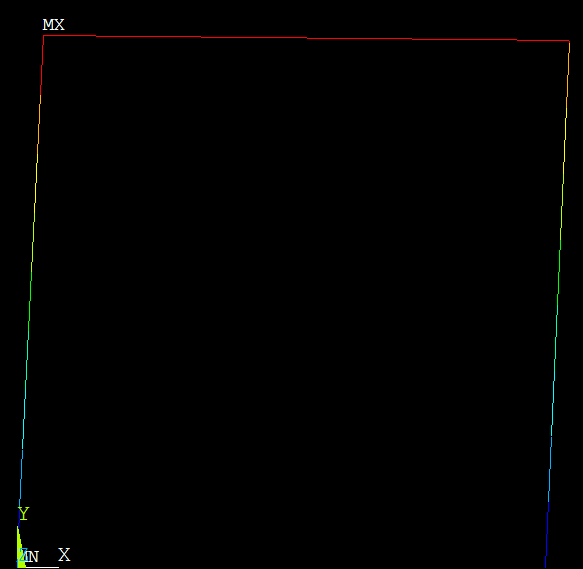
\includegraphics[width=8cm]{ScreenClip.png}
\end{center}

\section{Matlab程序}

\begin{verbatim}
E=2e7;
l=100;
A=10;
Iz=25;
P=10000;

Ke=[E*A/l,0,0,-E*A/l,0,0;
    0,12*E*Iz/l^3,6*E*Iz/l^2,0,-12*E*Iz/l^3,6*E*Iz/l^2;
    0,6*E*Iz/l^2,4*E*Iz/l,0,-6*E*Iz/l^2,2*E*Iz/l;
    -E*A/l,0,0,E*A/l,0,0;
    0,-12*E*Iz/l^3,-6*E*Iz/l^2,0,12*E*Iz/l^3,-6*E*Iz/l^2;
    0,6*E*Iz/l^2,2*E*Iz/l,0,-6*E*Iz/l^2,4*E*Iz/l];

Ke_local=cat(3,zeros(6),zeros(6),zeros(6));
for k=1:3
    Ke_local(:,:,k)=Ke;
end

Lambada(:,:,1)=[0,1,0,0,0,0;
                -1,0,0,0,0,0;
                0,0,1,0,0,0;
                0,0,0,0,1,0;
                0,0,0,-1,0,0;
                0,0,0,0,0,1];

Lambada(:,:,2)=[1,0,0,0,0,0;
                0,1,0,0,0,0;
                0,0,1,0,0,0;
                0,0,0,1,0,0;
                0,0,0,0,1,0;
                0,0,0,0,0,1];

Lambada(:,:,3)=[0,-1,0,0,0,0;
                1,0,0,0,0,0;
                0,0,1,0,0,0;
                0,0,0,0,-1,0;
                0,0,0,1,0,0;
                0,0,0,0,0,1];

Ke_global=cat(3,zeros(6),zeros(6),zeros(6));
for k=1:3
   Ke_global(:,:,k)=Lambada(:,:,k)'*Ke_local(:,:,k)*Lambada(:,:,k);
end

K=zeros(12);
for elem=1:3
    for r=1+(elem-1)*3:6+(elem-1)*3
        for c=1+(elem-1)*3:6+(elem-1)*3
            K(r,c)=K(r,c)+Ke_global(r-(elem-1)*3,c-(elem-1)*3,elem);
        end
    end
end

load=[0,0,0,P,0,0,0,0,0,0,0,0]';
delta=zeros(12,1);

delta(4:9,1:1)=linsolve(K(4:9,4:9),load(4:9,1:1));
load=K*delta;
for t=5:9
    load(t)=0;
end
\end{verbatim}

\end{document}





































